\section{Implementare}

\begin{frame}{Implementare: Arhitectură de Ansamblu} \pause
	\begin{itemize}
		\item Arhitectură de tip lider - subordonați \pause
		\item Servere construite pe fundația modulelor \pause
		\item Gruparea modulelor ca o linie de asamblare
	\end{itemize}
\end{frame}

\begin{frame}{Implementare: Module} \pause
	\begin{itemize}
	    \item Gestionarea serverelor subordonate
	    \item Etichetarea fișierelor și gestionarea seturilor de date
		\item Extragerea atributelor din fișiere
		\item Preprocesarea atributelor
		\item Gestionarea modelelor de inteligență artificială
		\item Gestionarea serverelor subordonate
	\end{itemize}
\end{frame}

\begin{frame}{Implementare: Gestionarea Serverelor Subordonate}
	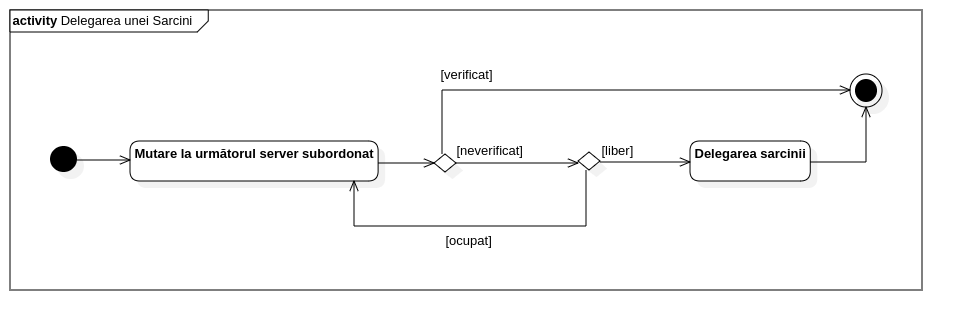
\includegraphics[width=\textwidth, center]{components/images/diagrams/activity_diagram_task_delegation.png}
    \captionsetup{justification=centering,margin=1cm}
    \captionof{figure}{Arhitectura Modulului pentru Gestionarea Serverelor Subordonate}
\end{frame}

\begin{frame}{Implementare: Etichetarea Fișierelor și Gestionarea Seturilor de Date}
	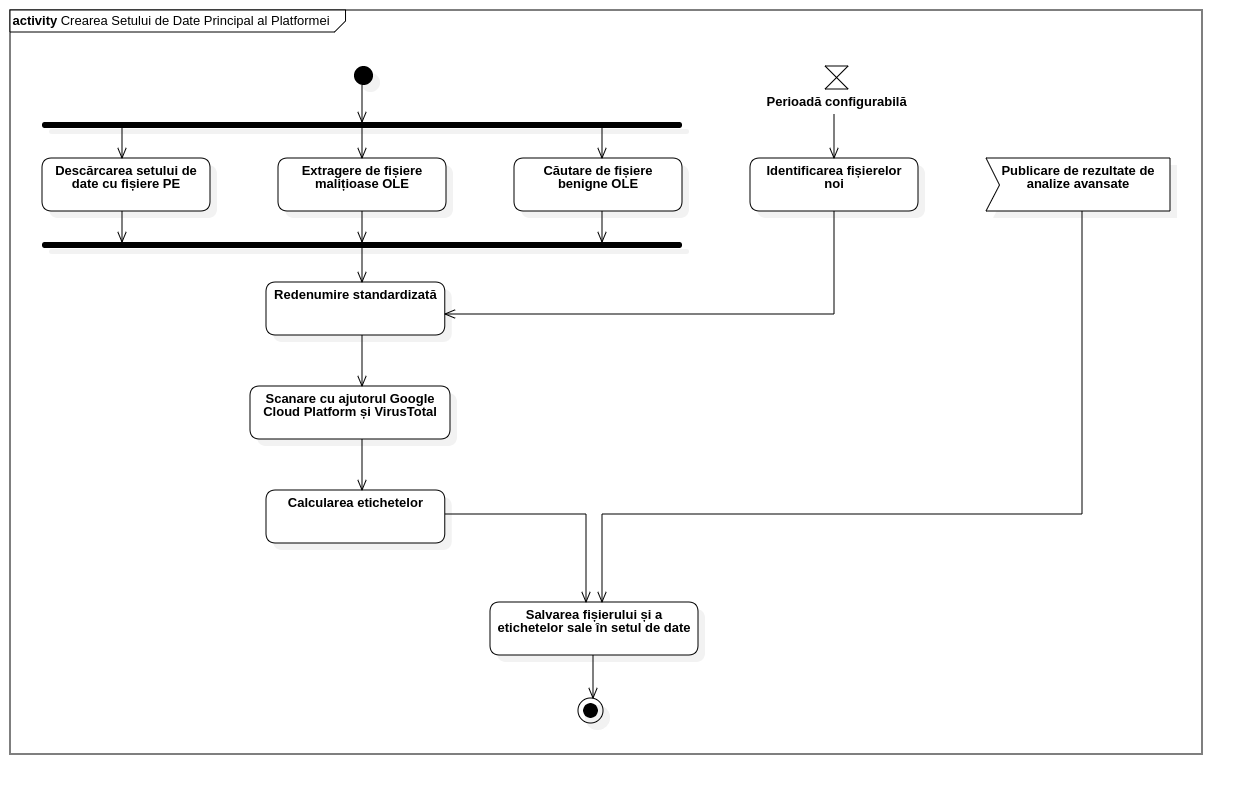
\includegraphics[width=0.8\textwidth, center]{components/images/diagrams/activity_diagram_dataset_creation.png}
    \captionsetup{justification=centering,margin=1cm}
    \captionof{figure}{Arhitectura Modulului pentru Etichetarea Fișierelor și Gestionarea Seturilor de Date}
\end{frame}

\begin{frame}{Implementare: Extragerea Atributelor din Fișiere}
	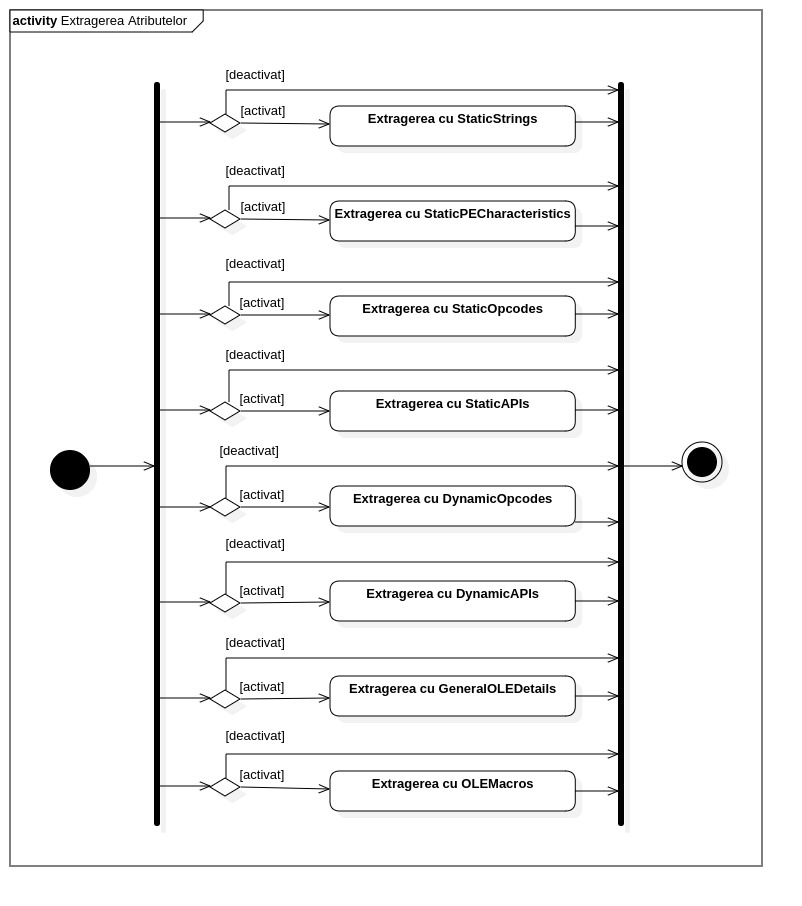
\includegraphics[width=0.5\textwidth, center]{components/images/diagrams/activity_diagram_attribute_extraction.png}
    \captionsetup{justification=centering,margin=1cm}
    \captionof{figure}{Arhitectura Modulului pentru Extragerea Atributelor din Fișiere}
\end{frame}

\begin{frame}{Implementare: Preprocesarea Atributelor}
	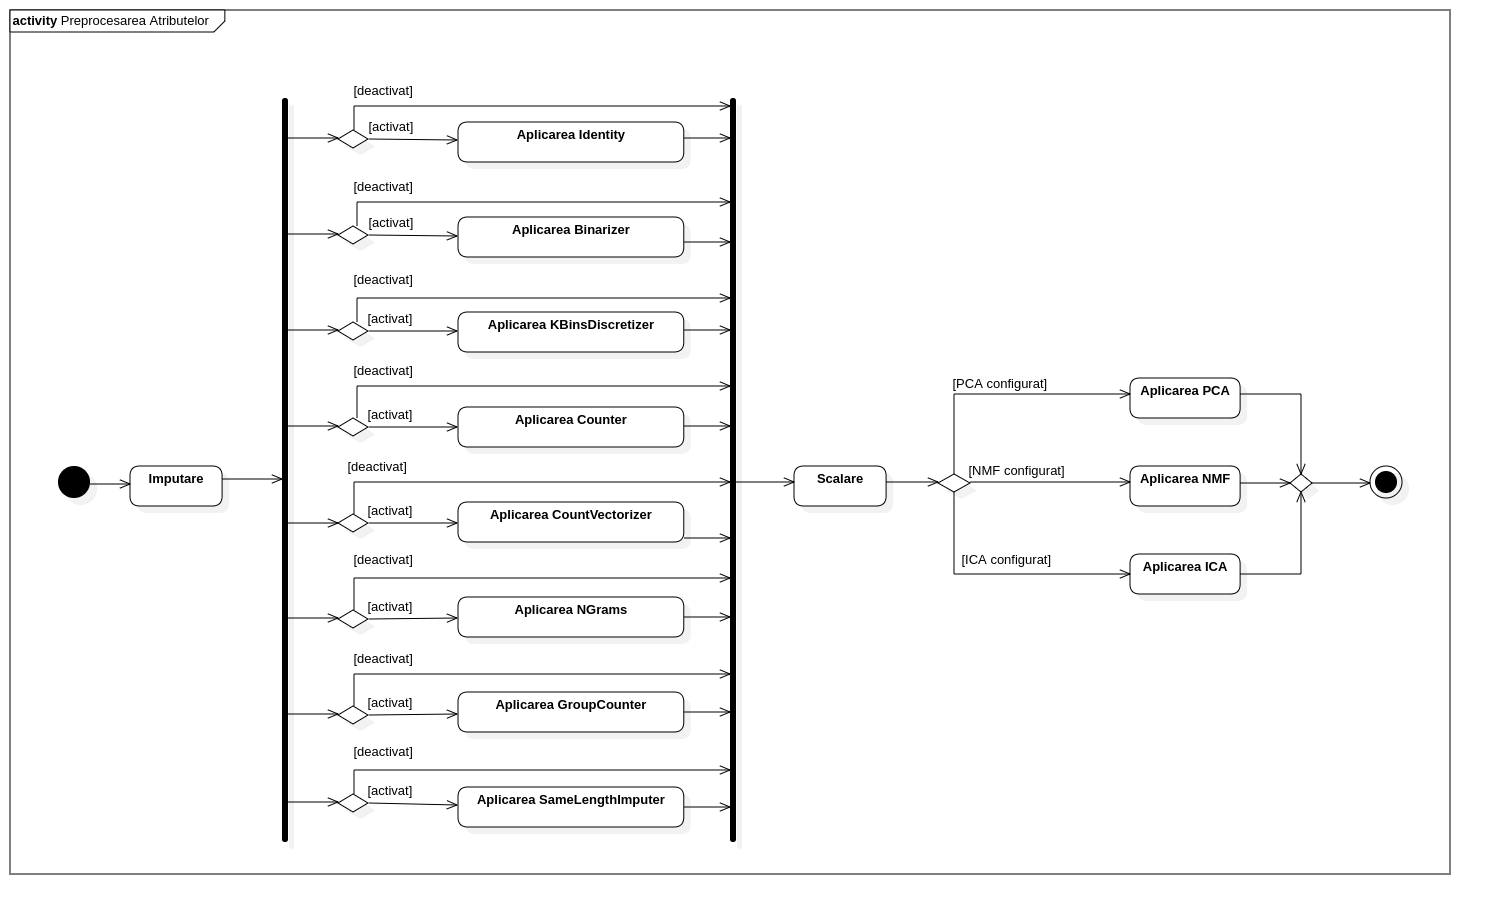
\includegraphics[width=0.8\textwidth, center]{components/images/diagrams/activity_diagram_attribute_preprocessing.png}
    \captionsetup{justification=centering,margin=1cm}
    \captionof{figure}{Arhitectura Modulului pentru Preprocesarea Atributelor}
\end{frame}

\begin{frame}{Implementare: Gestionarea Modelelor de Inteligență Artificială}
	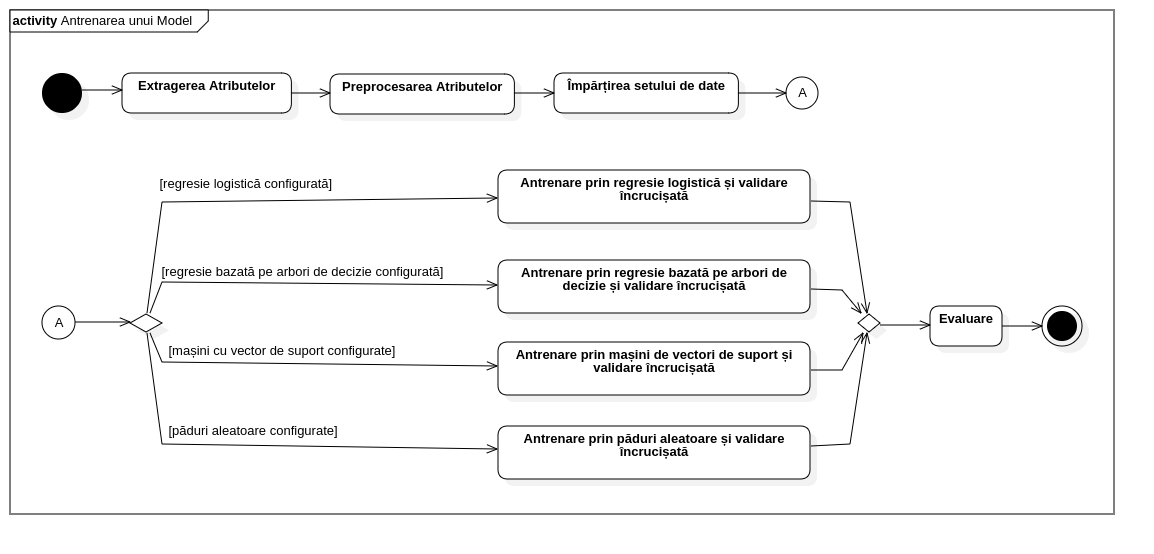
\includegraphics[width=0.9\textwidth, center]{components/images/diagrams/activity_diagram_model_training.png}
    \captionsetup{justification=centering,margin=1cm}
    \captionof{figure}{Arhitectura Modulului pentru Gestionarea Modelelor de Inteligență Artificială}
\end{frame}

\begin{frame}{Implementare: Arhitectura de Servere}
	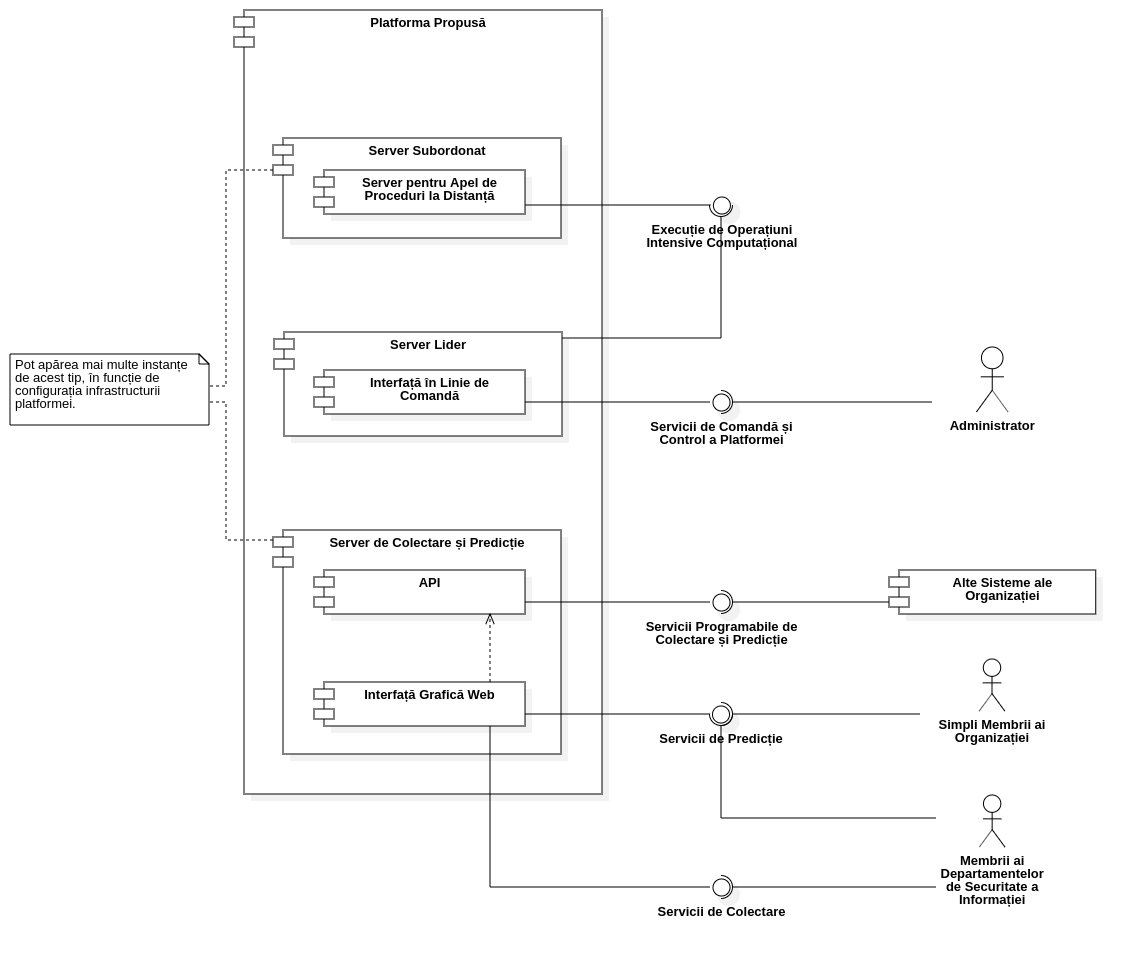
\includegraphics[width=0.7\textwidth, center]{components/images/diagrams/component_diagram_servers.png}
    \captionsetup{justification=centering,margin=1cm}
    \captionof{figure}{Arhitectura de Servere a Platformei}
\end{frame}

\extras{
    \begin{frame}{Implementare: Alte Detalii} \pause
        \begin{itemize}
            \item Tehnologii folosite
            \vspace{0.3cm}
            \begin{table}[!htb]
    \centering
        \begin{tabular}{ cccccc }
            
\includegraphics[width=20pt,margin=0pt 1ex 0pt 1ex,valign=m]{components/images/logos/ghidra.png} & 
            
\includegraphics[width=20pt,margin=0pt 1ex 0pt 1ex,valign=m]{components/images/logos/virustotal.png} &
            
\includegraphics[width=20pt,margin=0pt 1ex 0pt 1ex,valign=m]{components/images/logos/qiling.png} & 
            
\includegraphics[width=20pt,margin=0pt 1ex 0pt 1ex,valign=m]{components/images/logos/pandas.png} & 
            
\includegraphics[width=20pt,margin=0pt 1ex 0pt 1ex,valign=m]{components/images/logos/sklearn.png} & 
            
\includegraphics[width=20pt,margin=0pt 1ex 0pt 1ex,valign=m]{components/images/logos/yaml.png} \\
            
\includegraphics[width=15pt,margin=0pt 1ex 0pt 1ex,valign=m]{components/images/logos/python.png} & 
            
\includegraphics[width=20pt,margin=0pt 1ex 0pt 1ex,valign=m]{components/images/logos/docker.png} &
            
\includegraphics[width=20pt,margin=0pt 1ex 0pt 1ex,valign=m]{components/images/logos/compose.png} & 
            
\includegraphics[width=15pt,margin=0pt 1ex 0pt 1ex,valign=m]{components/images/logos/bash.png} & 
            
\includegraphics[width=15pt,margin=0pt 1ex 0pt 1ex,valign=m]{components/images/logos/github.png} & 
            
\includegraphics[width=20pt,margin=0pt 1ex 0pt 1ex,valign=m]{components/images/logos/latex.png}
        \end{tabular}
    \label{tab:logos}
\end{table}
            \vspace{0.3cm} \pause
    	    \item Aspecte considerate \pause
    	    \begin{itemize}
        	    \item Calcul distribuit și paralel \pause
        	    \item Containerizare \pause
        	    \item Documentare \pause
        	    \item Configurabilitate
        	\end{itemize}
    	\end{itemize}
    \end{frame}
}